 \chapter{Software utilizado}

\thispagestyle{plain}
\renewcommand{\tablename}{Tabla}

\section{Introducción}

En este capitulo se recopilará el software empleado en el desarrollo del proyecto. Se procede a dividir el capítulo creando secciones para cada programa y exponiéndolos brevemente.

\section{Arduino IDE}

El entorno de desarrollo integrado (IDE) de Arduino es una aplicación multiplataforma (Linux, Windows y macOS) que permite escribir y cargar programas en placas Arduino. Admite lenguajes de programación como C y C++. El programa solo requiere de dos funciones básicas para funcionar, el \textit{setup} y \textit{loop}.

\begin{figure}[H]
    \centering
    
\includegraphics[width=0.25\linewidth]{imagenes/Logo Arduino.png}
    \caption{Logotipo Arduino. \cite{Arduino}}
    \label{fig:logo-Arduino}
\end{figure}

En este proyecto se utiliza esta IDE para desarrollar códigos básicos que permitan una primera toma de contacto de la comunicación CAN Bus entre la placa y el motor.

\section{TeraTerm}

TeraTerm es un software gratuito que permite emular sistemas de comunicación. 

\begin{figure}[H]
    \centering
    
\includegraphics[width=0.25\linewidth]{imagenes/Logo TeraTerm.png}
    \caption{Logotipo TeraTerm. \cite{TeraTerm}}
    \label{fig:logo-TeraTerm}
\end{figure}

El motor GIM8108 V3 incluye un puerto UART el cual permite acceder al firmware del motor. Para realizar esta conexión es necesario la utilización de un convertidor USB a TTL UART, decidiéndose utilizar el DSD TECH SH-U09C (figura \ref{fig:USB-UART}).

\begin{figure}[H]
    \centering
    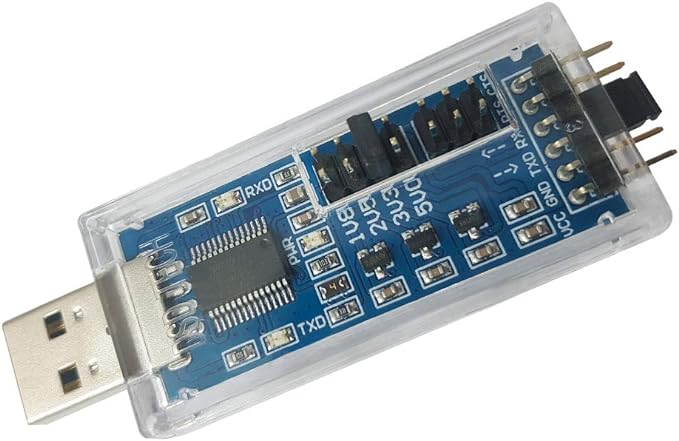
\includegraphics[width=0.5\linewidth]{imagenes/USB-UART.png}
    \caption{Convertidor de USB a TTL UART. \cite{TTL}}
    \label{fig:USB-UART}
\end{figure}

Una vez realizado el conexionado físico se procede a la configuración del interfaz serie en el ordenador. Para ello se establece una nueva conexión serie en TeraTerm con el puerto de comunicación del convertidor USB. Dicha conexión deberá ser configurada a \textit{921600 baud, 8 bits, 1 stop bit y no parity bits}.

\begin{figure}[H]
    \centering
    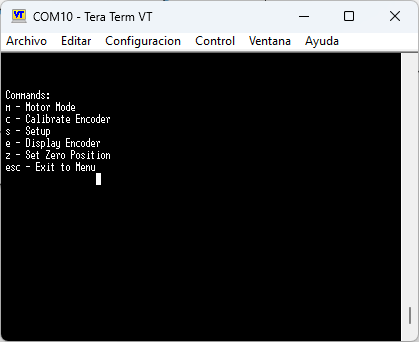
\includegraphics[width=0.75\linewidth]{imagenes/TeraTerm - Motor Menu.png}
    \caption{Menu (TeraTerm).}
    \label{fig:TeraTerm-MotorMenu}
\end{figure}

Este menú permite realizar las siguientes acciones sobre el motor:
\begin{itemize}
    \item \textit{Motor Mode}: En este modo el motor recibirá posición/velocidad/torque a través del CAN y enviará la posición real, velocidad y corriente.
    \item \textit{Calibrate Encoder}: Este proceso realiza el calibrado del sensor de posición del rotor. 
    \item \textit{Setup}: Permite el ajuste de  ciertos parámetros internos del motor (figura \ref{fig:TeraTerm-MotorSetup}).
    \item \textit{Display Encoder}: Muestra en tiempo real la lectura de los encoders (ángulo en radianes y cuenta). 
    \item \textit{Set Zero Position}: Sitúa a cero la posición actual del encoder.
\end{itemize}

\begin{figure}[H]
    \centering
    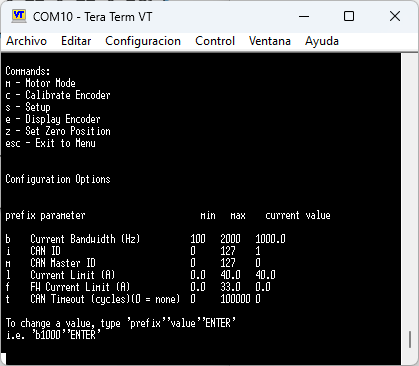
\includegraphics[width=0.75\linewidth]{imagenes/TeraTerm - Motor Setup.png}
    \caption{Setup (TeraTerm).}
    \label{fig:TeraTerm-MotorSetup}
\end{figure}

\section{MATLAB}

MATLAB es una plataforma de programación y cálculo numérico utilizada por millones de ingenieros y científicos para analizar datos, desarrollar algoritmos y crear modelos.

\begin{figure}[H]
    \centering
    
\includegraphics[width=0.5\linewidth]{imagenes/Logo MATLAB.png}
    \caption{Logotipo MATLAB \cite{MATLAB}.}
    \label{fig:logo-MATLAB}
\end{figure}

Para el desarrollo de este proyecto, son necesarios una serie de paquetes específicos que se deben añadir mediante el apartado \textit{Add-Ons} del propio MATLAB. Estos complementos son los siguientes:

\begin{itemize}
    \item MATLAB Support Package for Arduino Hardware
    \item Simulink Support Package for Arduino Hardware
    \item Embbedded Coder
    \item MATLAB Coder
    \item ROS Toolbox
    \item Simulink Coder
    \item Vehicle Network Toolbox
    \item Simulink Real-Time
\end{itemize}

\section{Simulink}

Simulink es un entorno de diagramas de bloque que se utiliza para diseñar sistemas con modelos multidominio, simular antes de implementar en hardware y desplegar sin necesidad de escribir código.

\begin{figure}[H]
    \centering
    
\includegraphics[width=0.5\linewidth]{imagenes/Logo Simulink.png}
    \caption{Logotipo Simulink \cite{Simulink}.}
    \label{fig:logo-Simulink}
\end{figure}

En este proyecto, Simulink es la herramienta más utilizada, puesto que es a partir de la cuál se crean los diversos modelos. Este, permite integrarlos en un solo proyecto, lo que facilita su exportación y organización.

\begin{figure}[H]
    \centering
    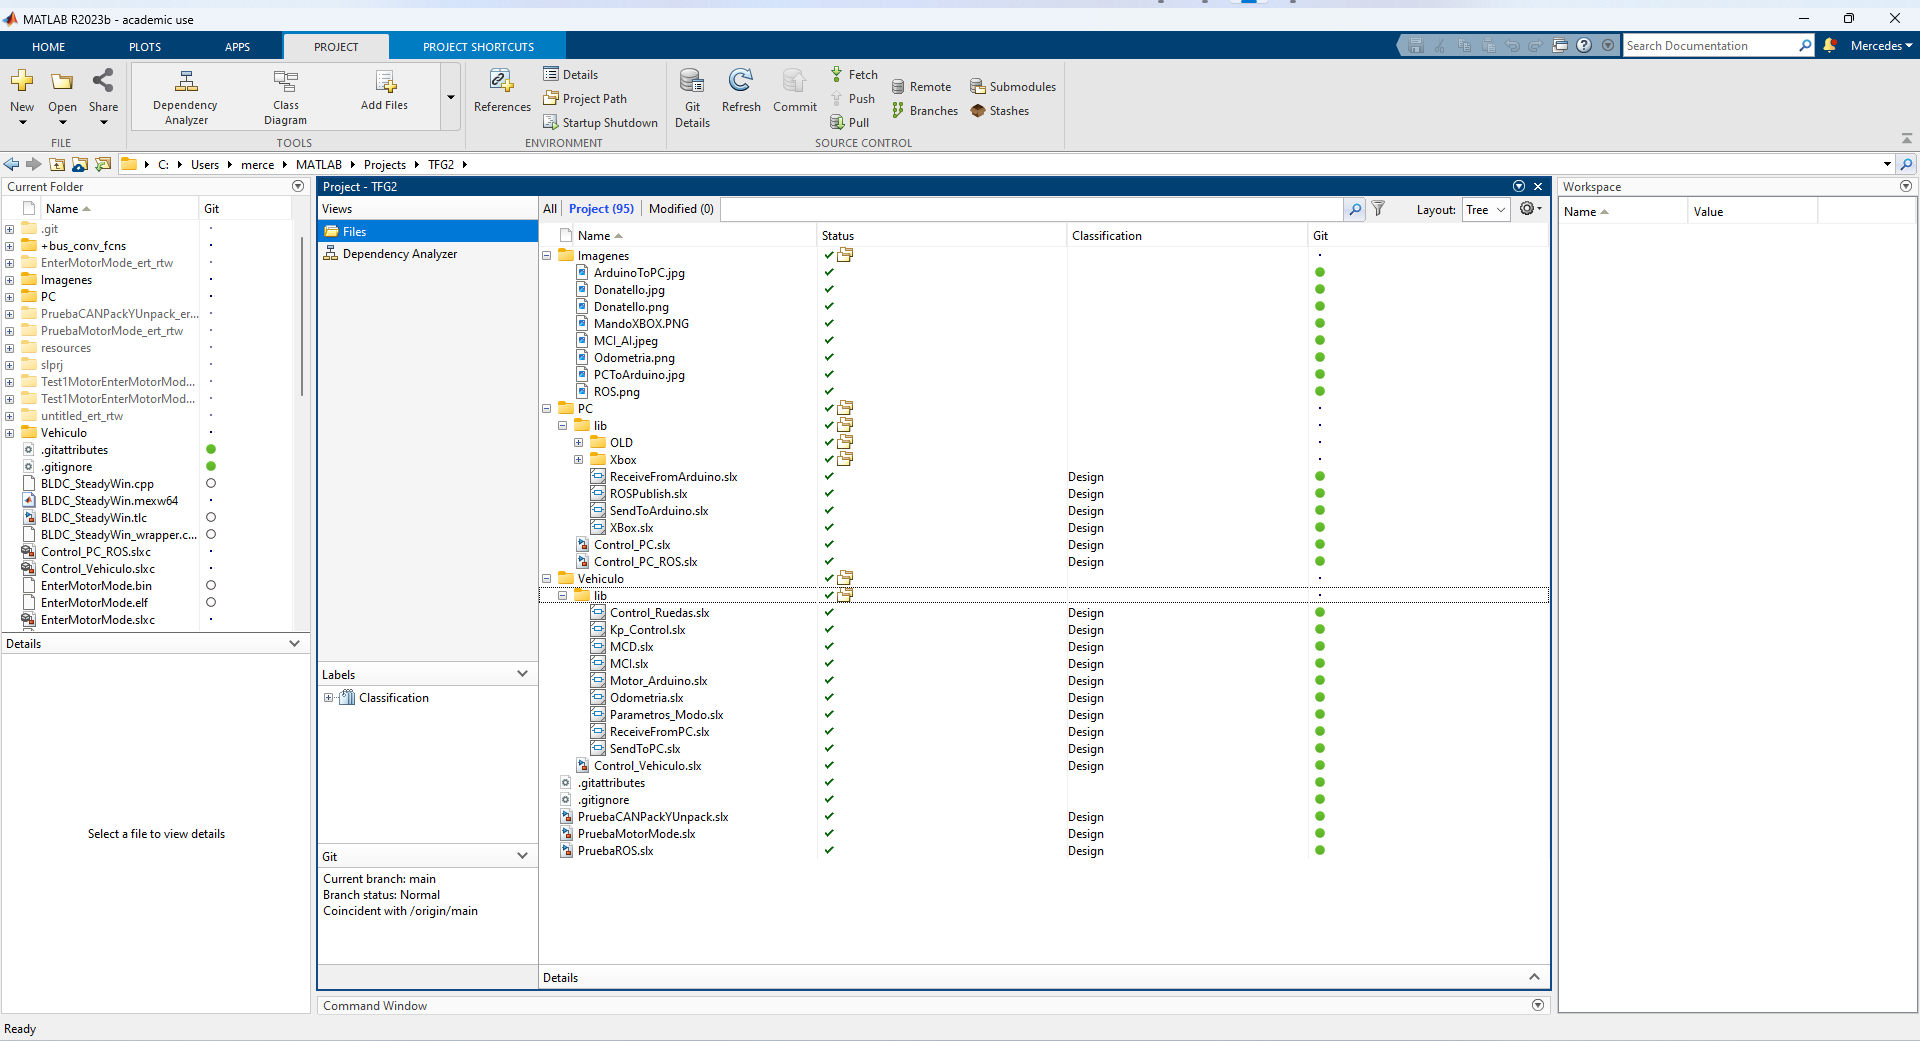
\includegraphics[width=0.75\linewidth]{imagenes/Proyecto - Simulink.png}
    \caption{Contenido proyecto en Simulink}
    \label{fig:Proyecto-Simulink}
\end{figure}

\section{GitHub}

GitHub es una plataforma de desarrollo colaborativo para alojar proyectos utilizando el sistema de control de versiones Git. Perteneciente a Microsoft desde el año 2018, se utiliza principalmente para la creación de código fuente de programas de ordenador. Además ofrece un servicio específico para estudiantes, conocido como Gitub Education, que permite a los estudiantes acceder a los beneficios de GitHub Pro.

\begin{figure}[H]
    \centering
    
\includegraphics[width=0.25\linewidth]{imagenes/Logo GitHub.png}
    \caption{Logotipo GitHub \cite{Wiki-GitHub}}
    \label{fig:logo-GitHub}
\end{figure}

Se decide utilizar GitHub por su facilidad de enlace con Simulink. Esto permitirá mantener un mayor control sobre las modificaciones realizadas en el proyecto de Simulink, además de permitir la colaboración. 

\begin{figure}[H]
    \centering
    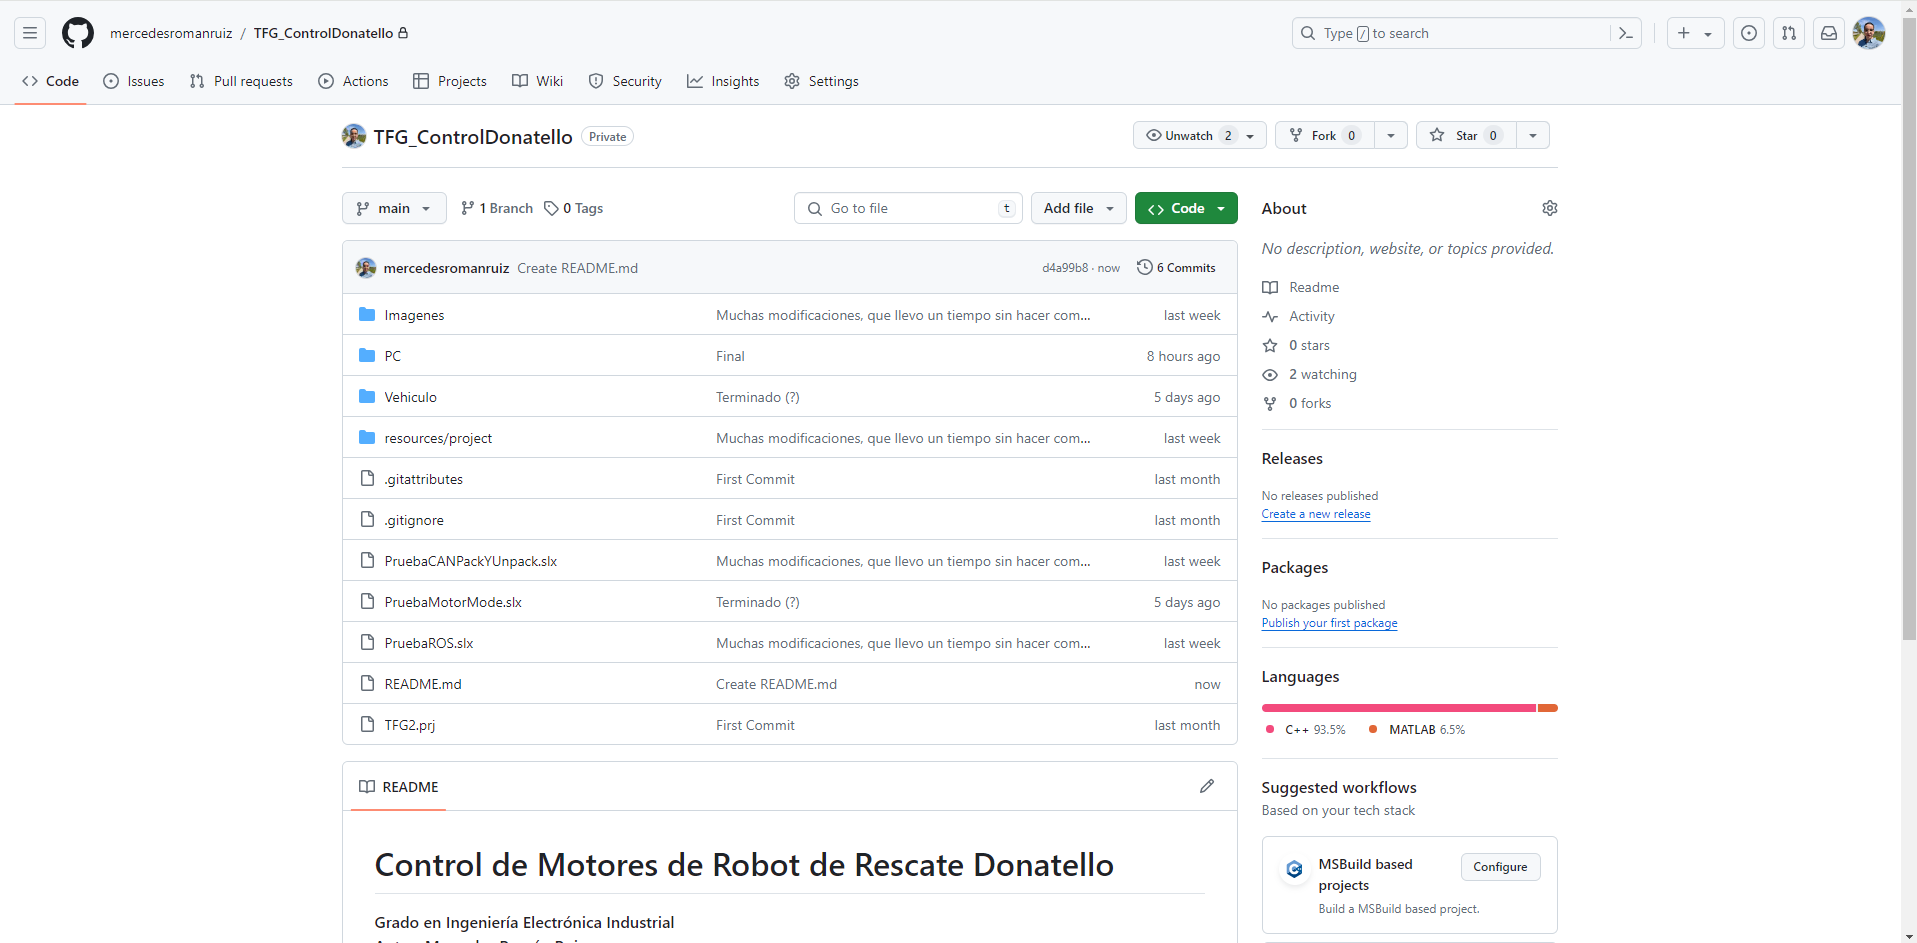
\includegraphics[width=0.75\linewidth]{imagenes/Proyecto - GitHub.png}
    \caption{Reposito del proyecto en GitHub}
\end{figure}

\section{ROS}
\textit{Robot Operating System}, también conocido como ROS, es un marco de trabajo flexible para el desarrollo de software de robótica. No es un sistema operativo en el sentido tradicional, sino una colección de herramientas, bibliotecas y convenciones diseñadas para simplificar la tarea de crear comportamientos complejos y robustos en robots. 

\begin{figure}[H]
    \centering
    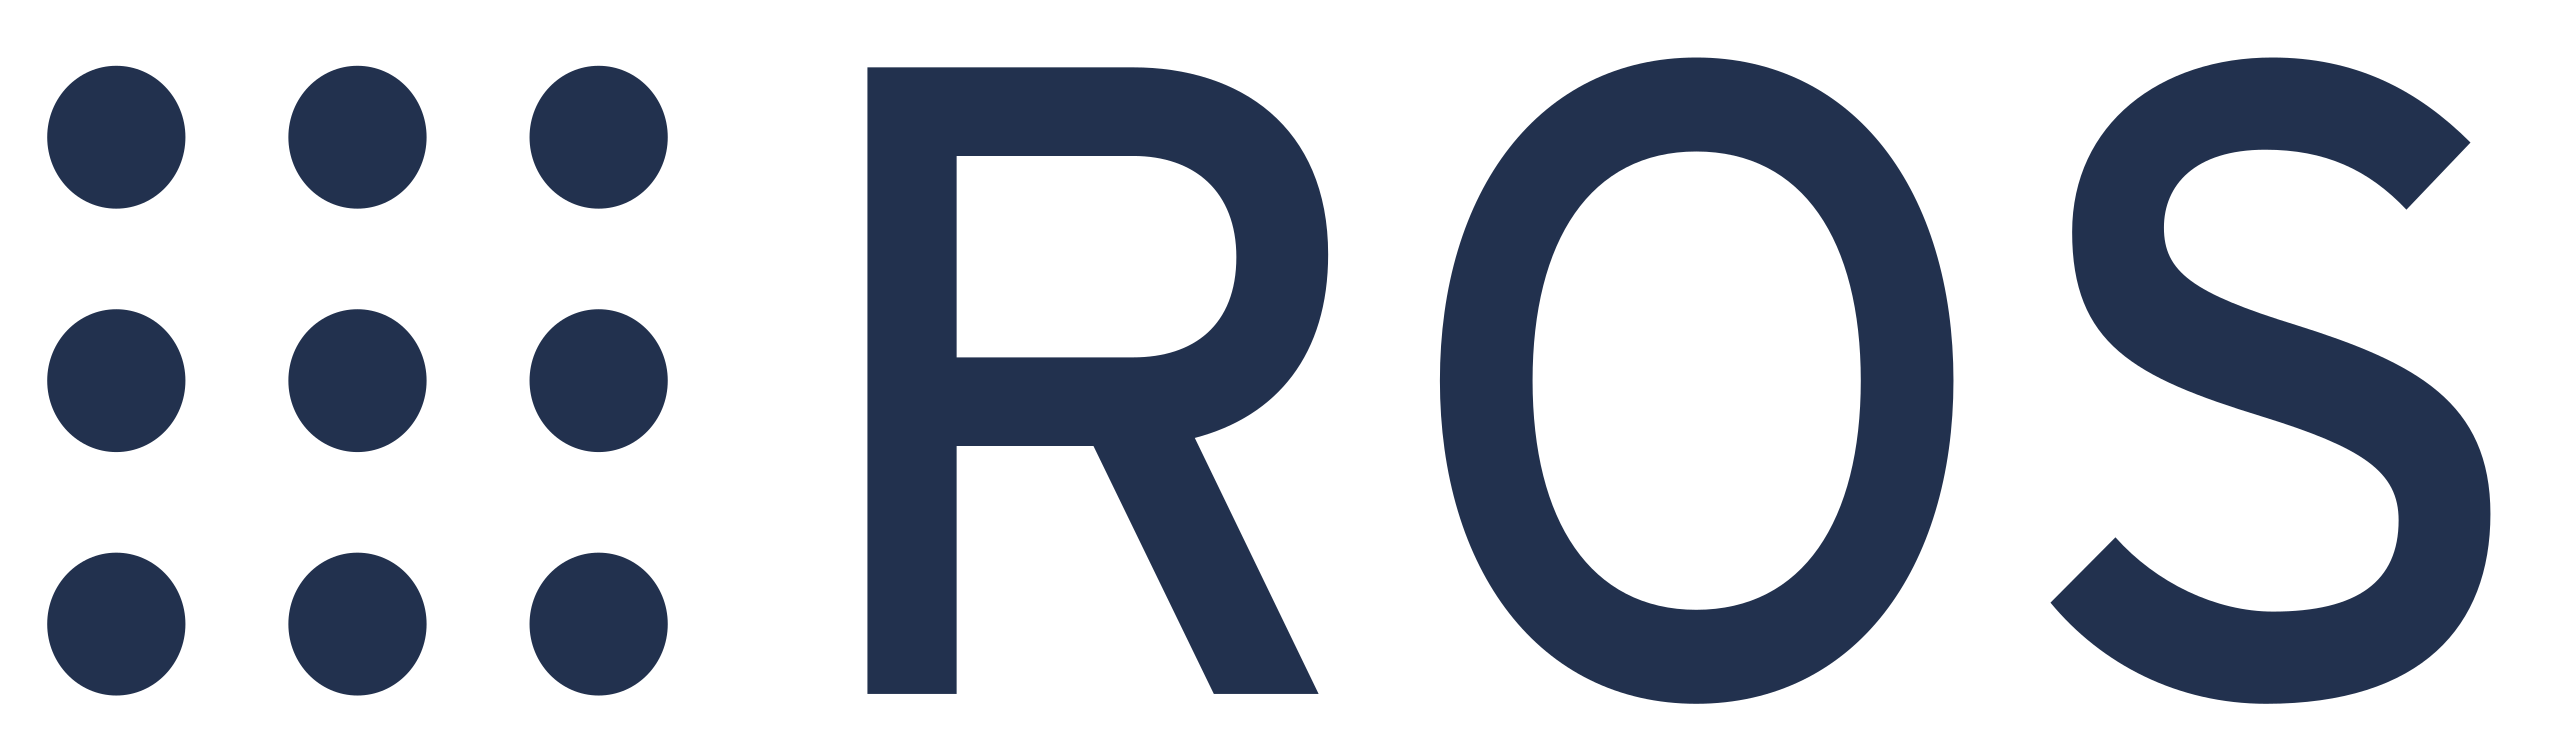
\includegraphics[width=0.5\linewidth]{imagenes/Logo ROS.png}
    \caption{Logotipo ROS \cite{ROS}}
    \label{fig:logo-ROS}
\end{figure}

ROS proporciona una infraestructura de comunicación entre procesos, que permite a los desarrolladores escribir software modular en forma de nodos que pueden intercambiar información mediante mensajes.

\begin{figure}[H]
    \centering
    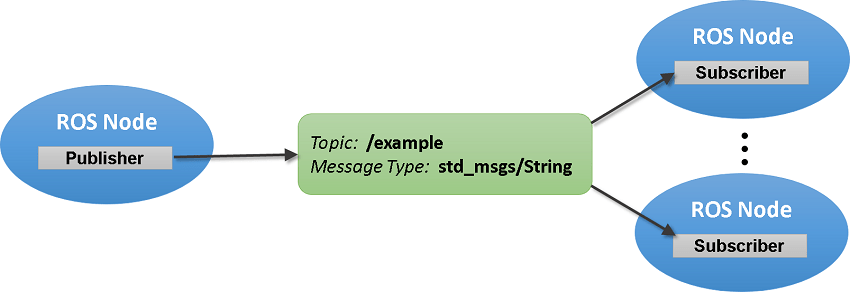
\includegraphics[width=0.75\linewidth]{imagenes/ROS Nodes - MathWorks.png}
    \caption{Ejemplo red ROS \cite{MathWorksROS}}
    \label{fig:ROS-Nodes}
\end{figure}

ROS2 es la segunda versión del framework de software ROS. Desarrollado por Open Robotics y una comunidad global de colaboradores, introduce mejoras significativas en términos de arquitectura, rendimiento y capacidades. En la siguiente tabla se elabora una comparativa entre ROS y ROS2:

\begin{table}[H]
    \centering
    \begin{tabular}{|p{4cm} | p{5cm} | p{6cm}|}
         \hline
         \rowcolor{lightgray}
         \textbf{Característica} & \textbf{ROS} & \textbf{ROS 2} \\
         \hline
         Modelo de Comunicación & Maestro central, TCPROS & Distribuido, DDS \\
         \hline
         Plataformas Soportadas & Linux & Linux, Windows, macOS \\
         \hline
         Soporte en Tiempo Real & No está diseñado para tiempo real & Soporte nativo para tiempo real \\
         \hline
         Seguridad & Carece de mecanismos integrados & Autenticación, cifrado, autorización (basados en DDS) \\
         \hline
         Gestión de Nodos & Gestión manual & Composición dinámica y modularidad \\
         \hline
         Comunidad y Paquetes & Comunicad establecida, amplia base de paquetes & Desarrollo activo, foco en mejoras y nuevas características \\
         \hline
         Interfaz de Línea de Comandos (CLI) & ROS (catkin\_make) & ROS 2 (colcon) \\
         \hline
         API de Cliente & rospy (Python), roscpp (C++) & rclpy (Python), rclcpp (C++) \\
         \hline
         Integración de Middleware & ROS Master y Slave (protocolo TCP/UDP) & DDS (Data Distribution Service) \\
         \hline
         Parámetros y Configuración & Parámetros gestionados por el nodo & Sistema de parámetros basado en DDS \\
         \hline
         Lanzamiento y Gestión de Procesos & Archivos de lanzamiento & Archivos de lanzamiento con sintaxis extendida y soporte para composiciones de nodos dinámicos \\
         \hline
         Compatibilidad con Versiones Anteriores & No compatible con ROS 2 & No compatible con ROS \\
         \hline
    \end{tabular}
    \caption{Tabla Comparativa ROS y ROS 2.}
\end{table}

%\blankpage